In this section, we calculate the time varying risk measures, which means to calculate risk measures based on rolling windows, such as 3 month rolling window. Then we get a series of risk measure. By examine how the series of risk measures vary over-time, we may discover some interesting facts about different risk measures.

\subsection{Time varying maximum drawdown}

$\textit{Maximum drawdown}$ is the largest cumulative loss from peak to trough. In the return path of length n, the maximum drawdown is defined by
\begin{equation}
\mathbf{\mu}(X_{T_n}) = \mathrm{max_{1 < i < j \leq n} max}({X_{t_i}-X_{t_j}, 0})
\end{equation}

Unlike VaR and ES, the empirical distribution of maximum drawdown is more sensitive to the time length of measurement. We calculate the maximum drawdown of various assets for different path length (3 months, 6 months, 1 year, 2 years, 5 years) separately. As shown in Figure \ref{fig: dmaxdd_RMZ}, the maximum drawdown distribution tends to be multi-mode and centered around several specific values when we move to longer period. And the mean increases as the period length increases. Figure \ref{fig: dist_mdd} shows the empirical distribution of maximum drawdown under 6 month rolling window for various assets. The maximum drawdown distribution tends to be negative skewed and the density curves seems to be unsmooth even under short rolling period as 6 month. Table \ref{table:tail_maxdrawdown} shows the tail mean of maximum drawdown distributions under different significant levels. Note that the tail mean of maximum drawdown increases as the rolling window increases.

%%%%%%%
\iffalse

\begin{figure}[h]
\caption{Empirical distribution of maximum drawdown under 6 month rolling window} 
\centering
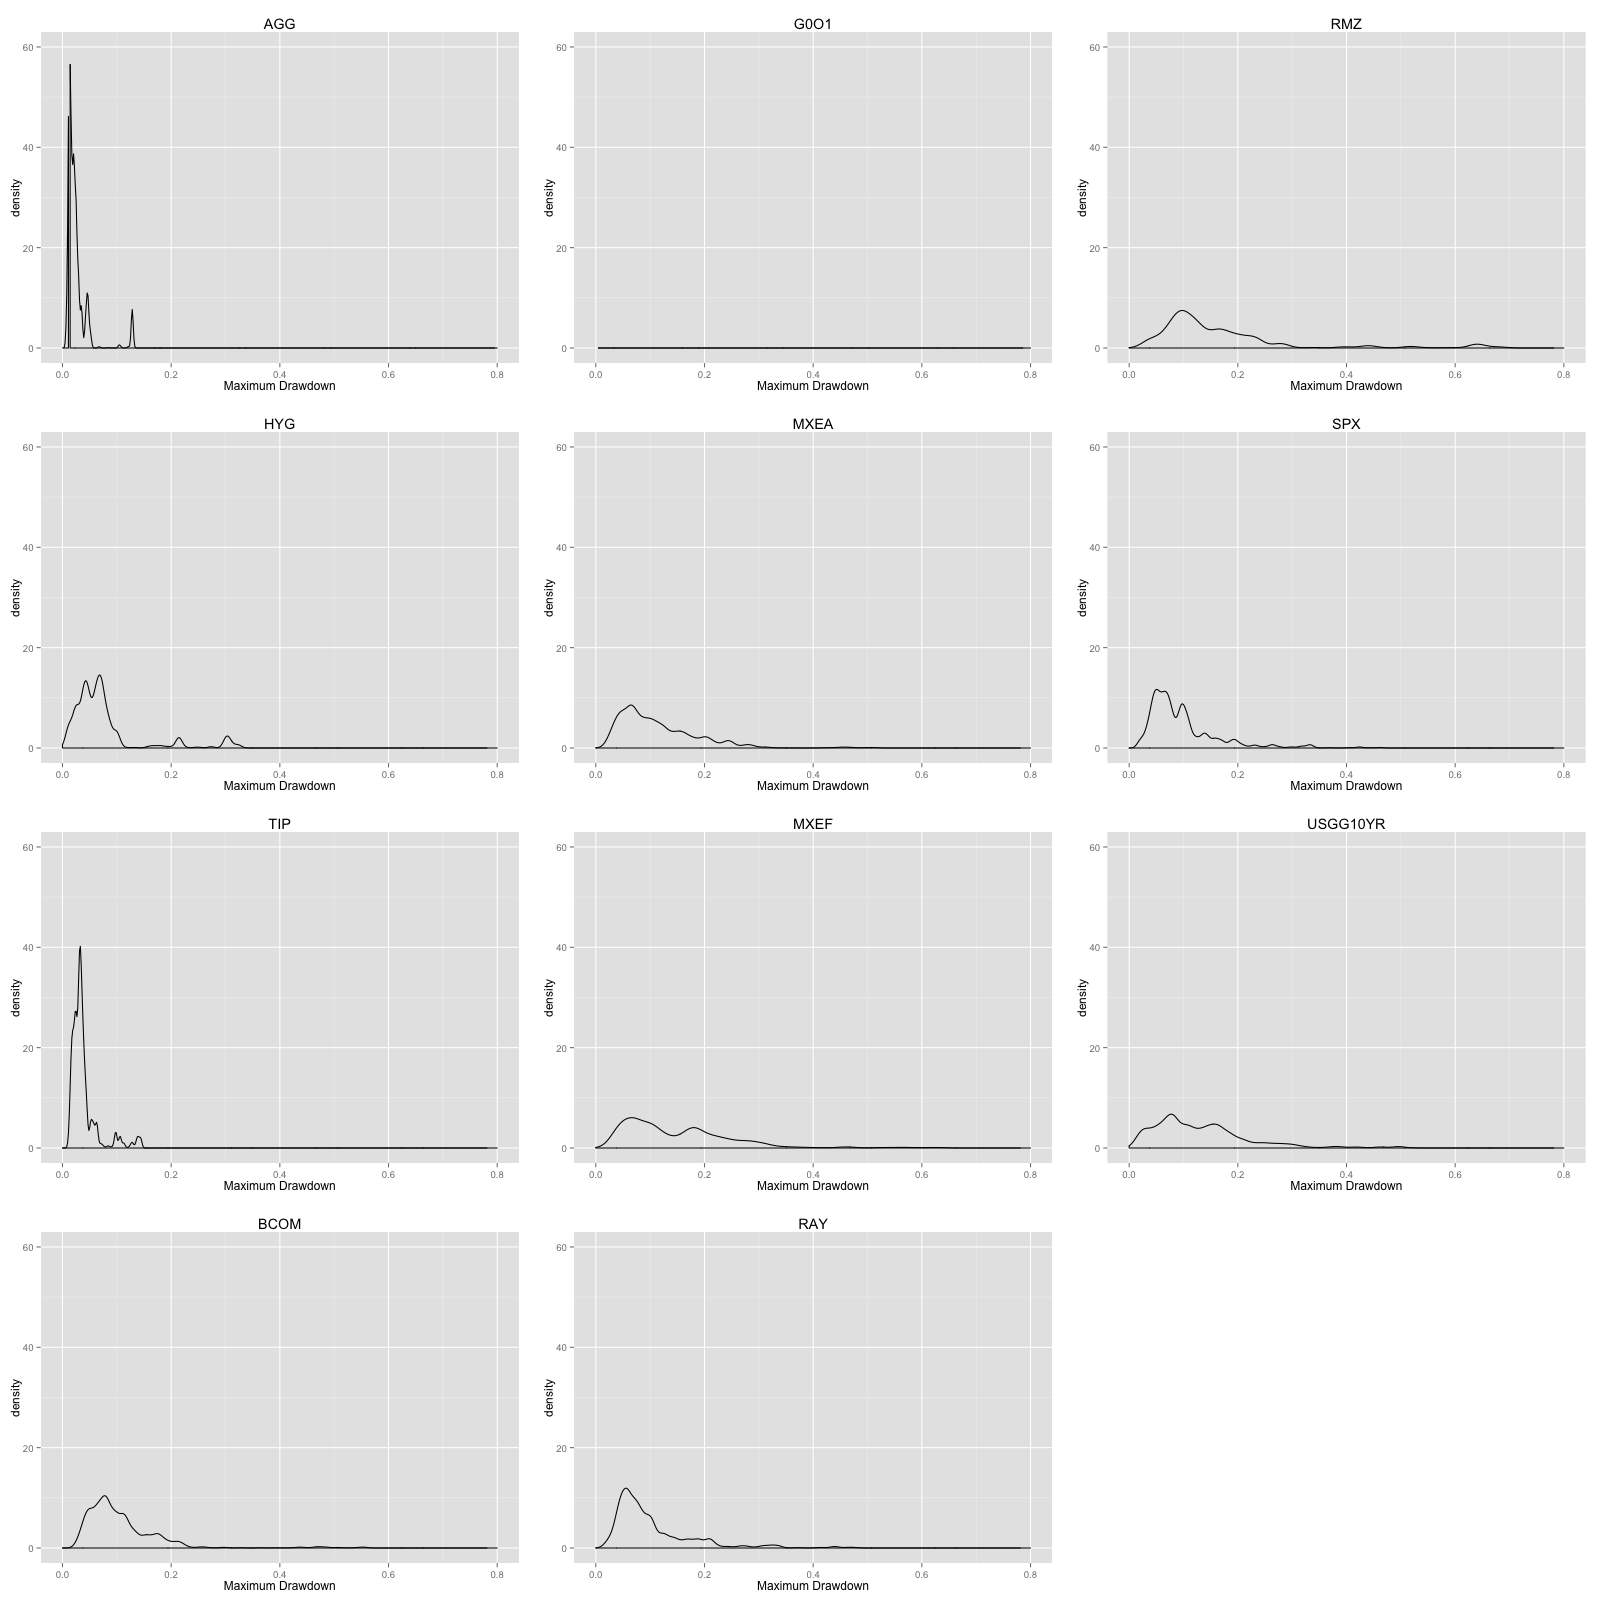
\includegraphics[width=15cm]{../results/maxdd_dist_mon6}
\label{fig: dist_mdd}
\end{figure}

\fi
%%%%%%%

\begin{figure}[h]
\caption{Maximum drawdown distribution of RMZ as rolling period increases} 
\centering 
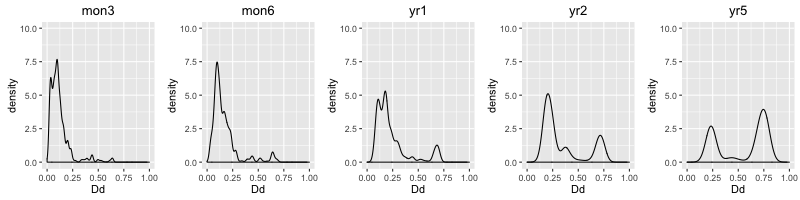
\includegraphics[width = 1\textwidth]{../results/maxdd_RMZ}
\label{fig: dmaxdd_RMZ}
\end{figure}

%%%%%%%
\iffalse

\begin{table}[!h]
\centering 
\caption{tail mean of maximum drawdown distribution under 3-month, 6-month, 1-year and 2-year rolling window} 
\begin{tabular}{ | r || r r r || r r r |} 
 \hline
 & & 3 month & & & 6 month & \\
Asset& 0.9 & 0.95 & 0.99 & 0.9 & 0.95 & 0.99  \\
  \hline \hline
AGG &  5.60 &  7.72 & 12.84 &  8.12 & 11.45 & 12.84\\ 
HYG & 18.41 & 24.07 & 29.67 & 26.43 & 30.77 & 32.26\\ 
TIP &  7.48 &  9.90 & 13.10 & 11.14 & 12.91 & 14.39\\ 
BCOM & 18.14 & 22.54 & 38.03 & 26.61 & 33.66 & 51.74\\ 
G0O1 &  0.10 &  0.145 &  0.26 &  0.14 &  0.23 &  0.26\\ 
MXEA & 20.39 & 23.73 & 33.32 & 27.21 & 31.79 & 47.11\\ 
MXEF & 26.21 & 30.80 & 48.03 & 36.35 & 43.30 & 59.63\\ 
RAY & 20.65 & 25.64 & 35.95 & 27.81 & 34.08 & 45.08\\ 
RMZ & 37.30 & 48.41 & 63.45 & 52.04 & 62.41 & 67.61\\ 
SPX & 18.35 & 22.67 & 32.46 & 25.18 & 30.65 & 40.69\\ 
USGG10YR & 23.28 & 28.11 & 41.83 & 32.78 & 39.00 & 49.28\\
 \hline \hline
 & & 1 year & & & 2 year & \\
Asset& 0.9 & 0.95 & 0.99 & 0.9 & 0.95 & 0.99  \\
  \hline \hline
AGG & 12.11 & 12.84 & 12.84 & 12.84 & 12.84 & 12.83\\ 
HYG & 33.15 & 34.20 &      & 34.24 & 34.25 &       \\ 
TIP & 13.73 & 14.50 & 14.57 & 14.57 & 14.57 &       \\ 
BCOM & 39.91 & 49.26 & 57.14 & 53.38 & 57.14 &       \\ 
G0O1 &  0.23 &  0.25 &  0.26 &  0.26 &  0.26 &  0.26\\ 
MXEA & 36.15 & 42.61 & 56.70 & 50.21 & 58.08 & 61.85\\ 
MXEF & 48.63 & 58.81 & 64.56 & 62.45 & 65.90 &       \\ 
RAY & 37.56 & 44.06 & 52.42 & 47.95 & 54.33 &       \\ 
RMZ & 67.09 & 69.86 & 70.02 & 73.70 & 74.56 & 74.92\\ 
SPX & 34.07 & 39.15 & 50.30 & 44.62 & 50.47 & 56.77\\ 
USGG10YR & 42.88 & 48.37 & 53.96 & 54.79 & 59.14 & 62.82\\
 \hline
\end{tabular}
\label{table:tail_maxdrawdown}
\end{table}

\fi
%%%%%%%

\subsection{Time varying volatility, VaR and ES}

Figure \ref{fig: variance6mon}, \ref{fig: VaR6mon} and \ref{fig: ES6mon} show the time varying volatility, VaR and ES based on 6-month rolling window (significance level = 0.95) for different assets. For every single asset, three risk measures seems to have similar pattern with each other. We further look at this similarity by calculate the correlation between different risk measures.

%%%%%%%
\iffalse

\begin{figure}[h]
\caption{Volatility under 6-month rolling window} 
\centering 
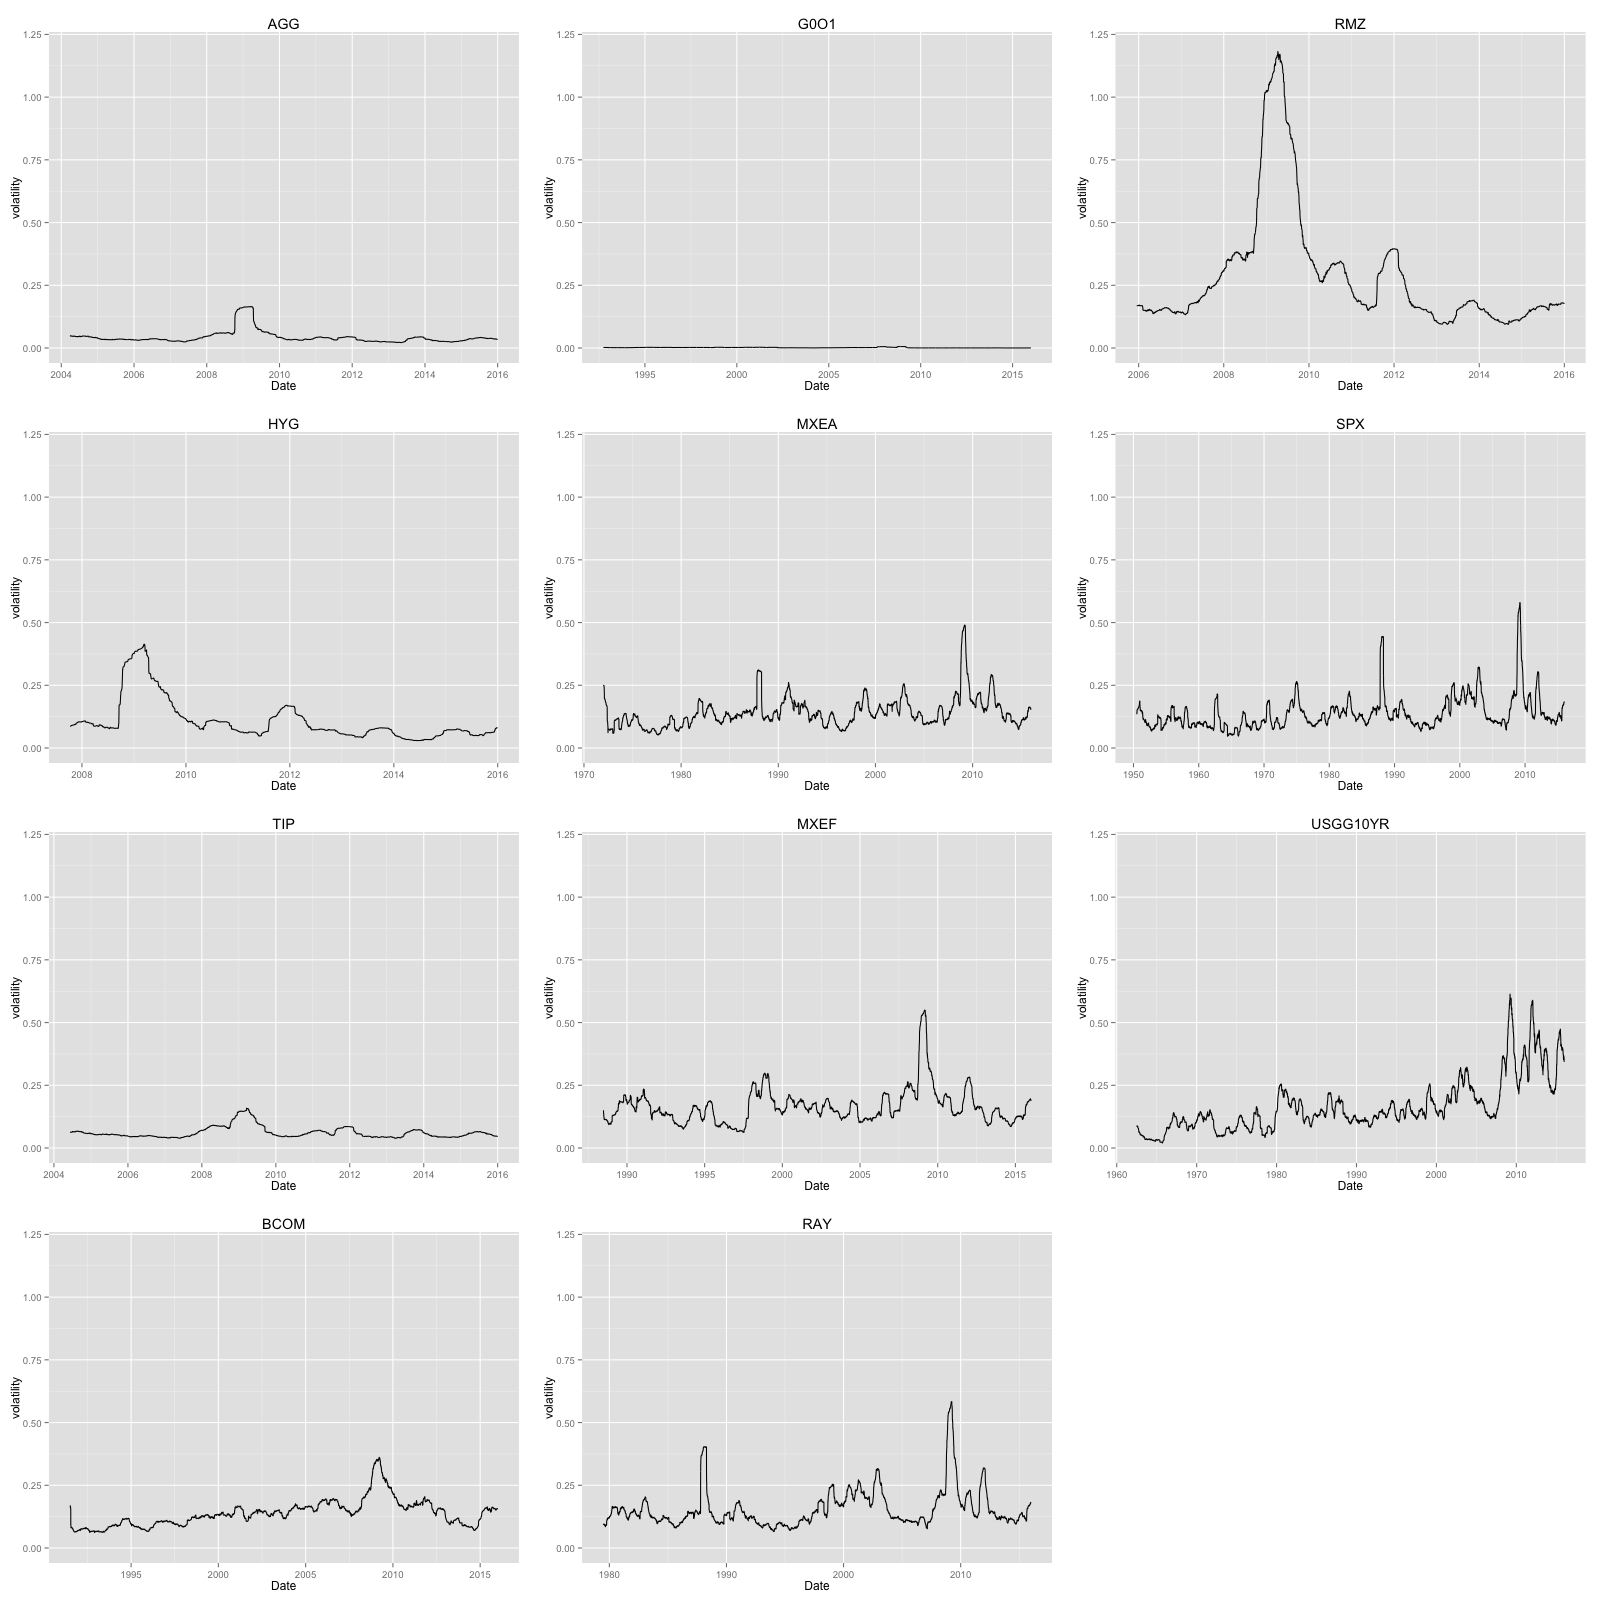
\includegraphics[width=15cm]{../results/volatility6mon}
\label{fig: variance6mon}
\end{figure}

\begin{figure}[h]
\caption{VaR(\%) (significance level = 0.95) under 6-month rolling window}
\centering 
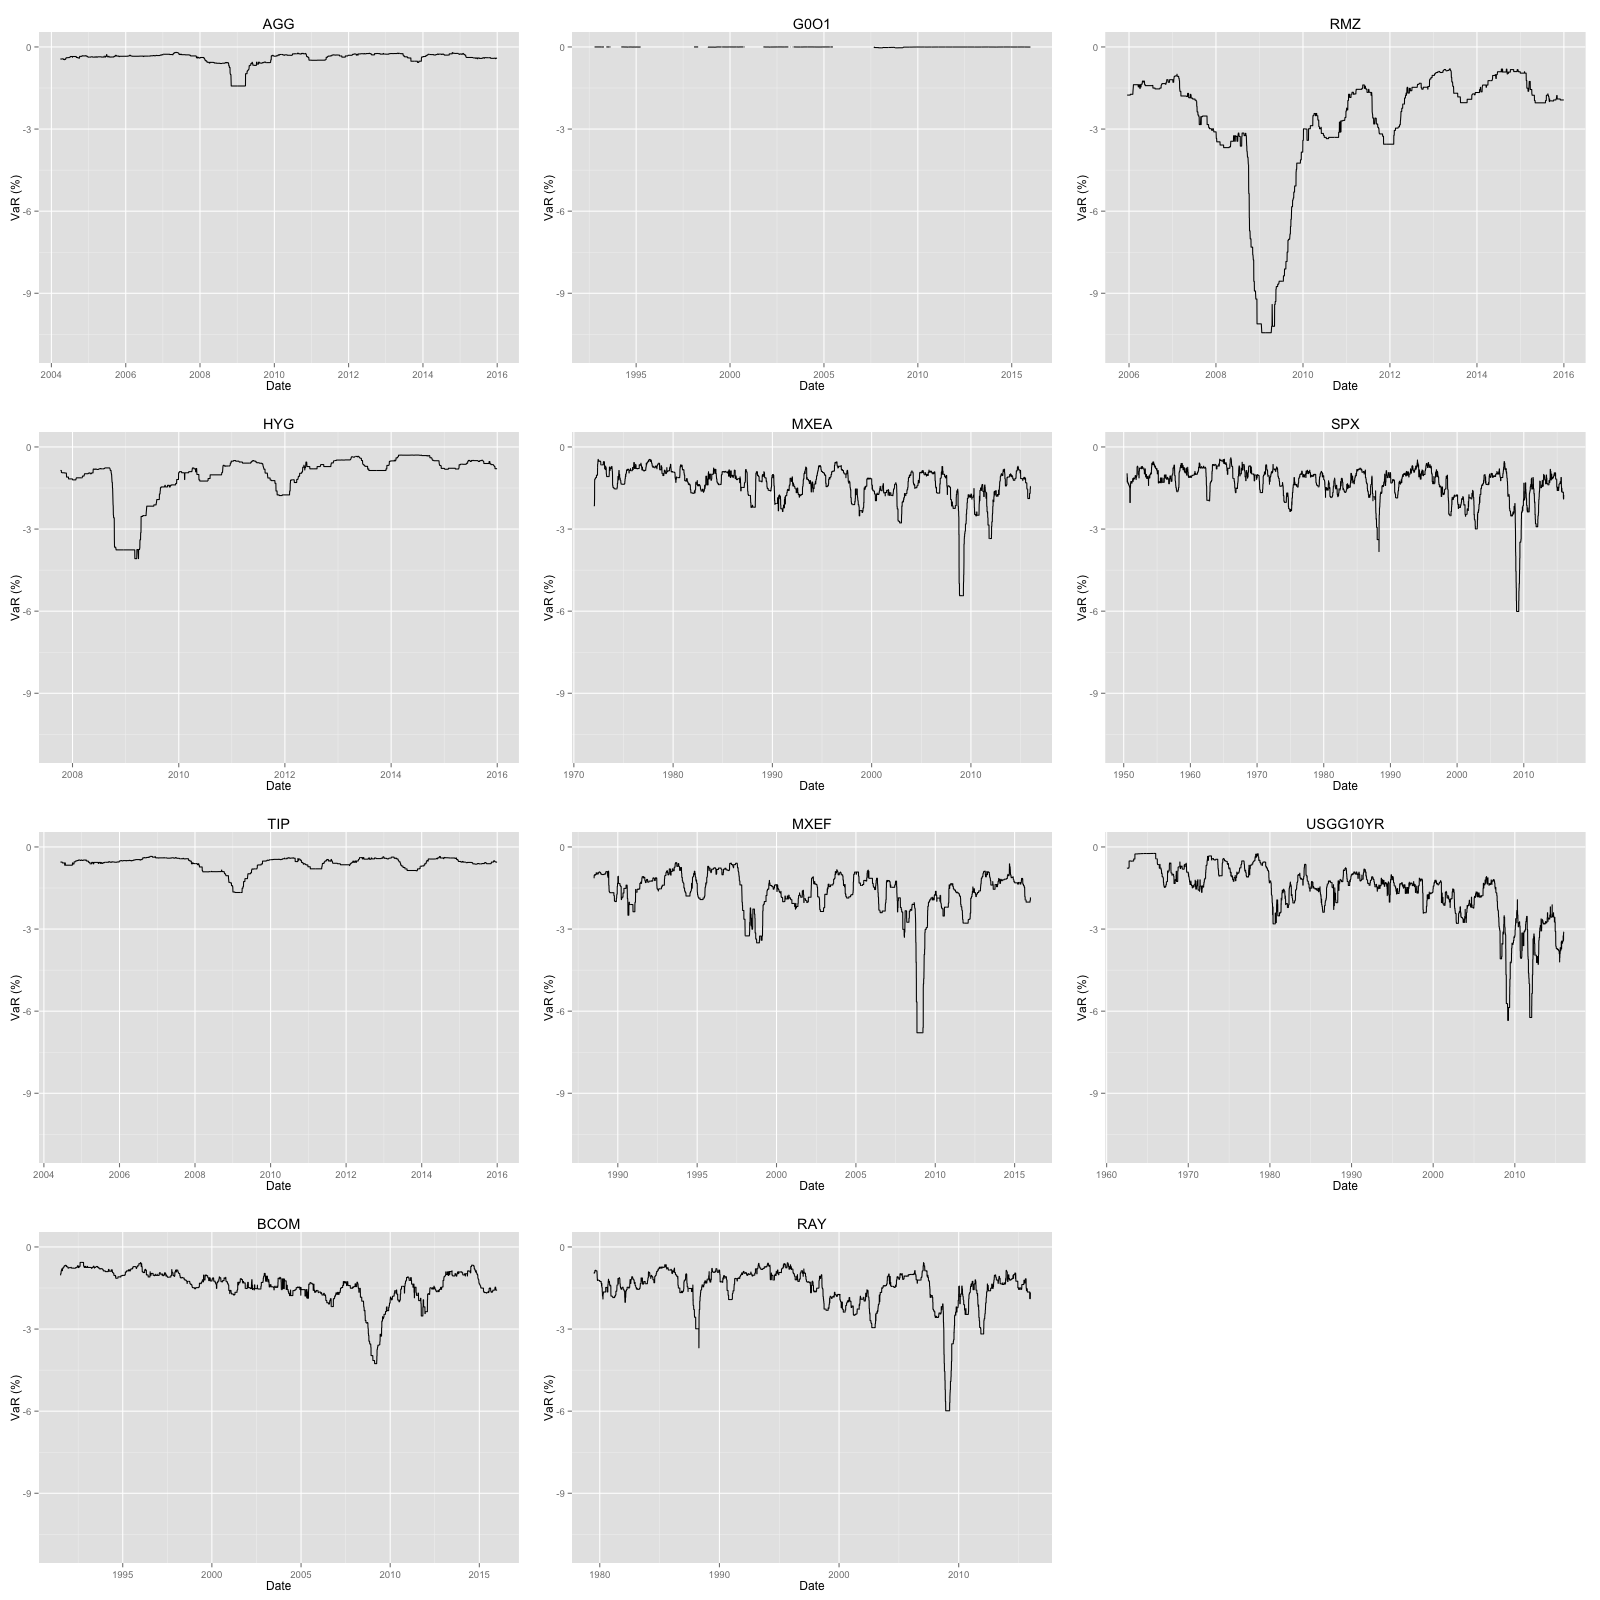
\includegraphics[width=15cm]{../results/VaR6mon_scaled}
\label{fig: VaR6mon}
\end{figure}

\begin{figure}[h]
\caption{ES(\%) (significance level = 0.95) under 6-month rolling window} 
\centering 
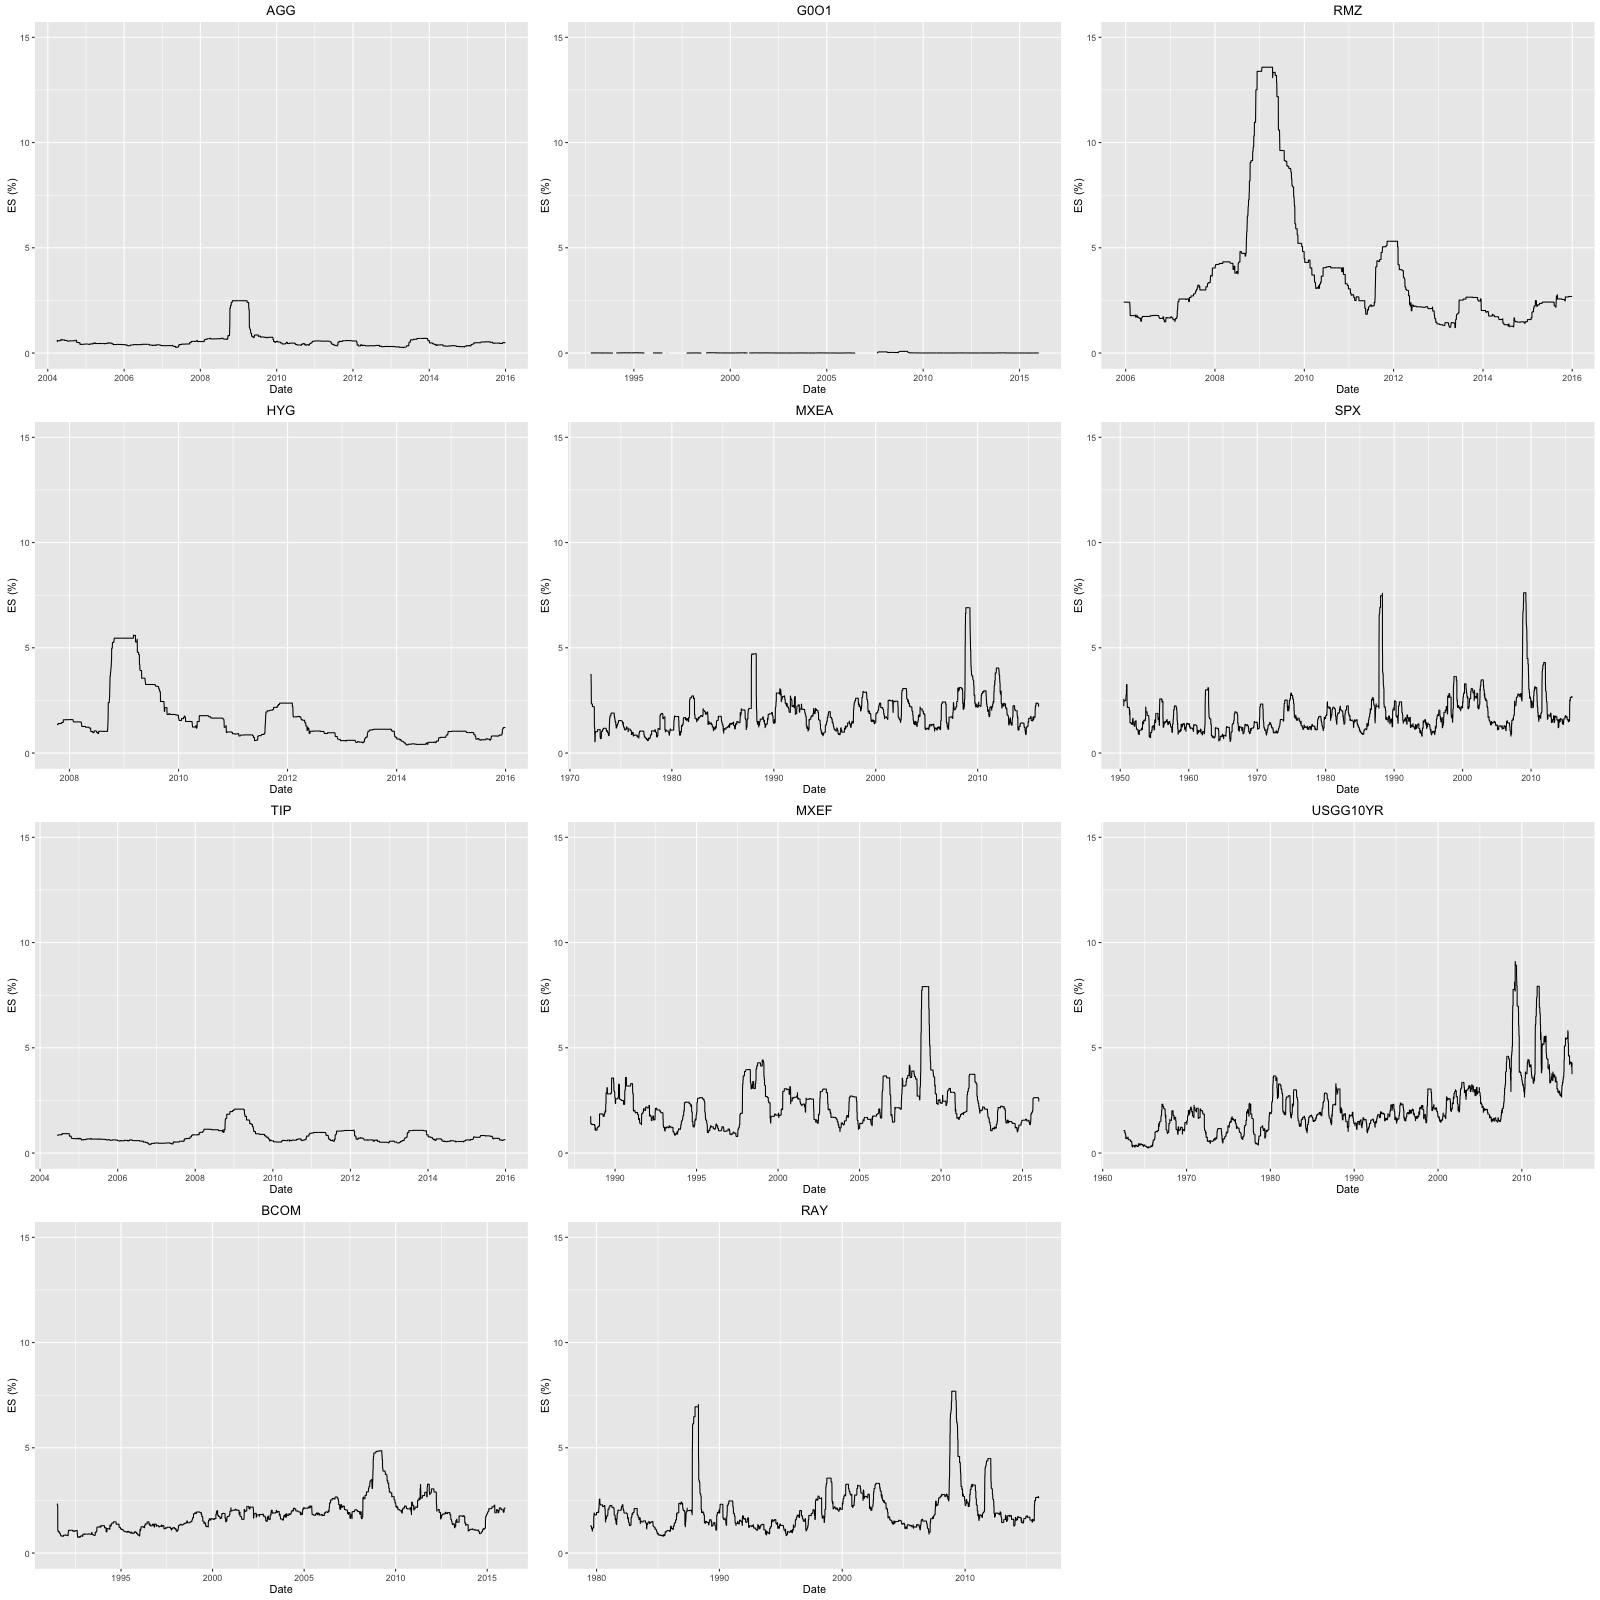
\includegraphics[width=15cm]{../results/ES6mon_scaled}
\label{fig: ES6mon}
\end{figure}

\fi
%%%%%%%

Table \ref{table:corrRiskMeasure} shows correlation between each pair of risk measures including VaR ($\alpha = 0.95$), ES ($\alpha = 0.95$), volatility and maximum drawdown. The correlation is calculated based on 6-month rolling risk measures. Among them, VaR, ES and volatility are closely related with each other, with average correlations over 95\%. Maximum drawdown has strong but comparatively weaker correlation with the other three. In general, these risk measures are all closely correlated. Figure \ref{fig: risk_meausre_RMZ} shows the comparison of the four risk measures calculated based on rolling windows for asset RMZ. Their pattens turned out to be very similar.

\begin{table}[h]
\caption{Correlation between risk measures}
\centering 
\begin{tabular}{ p{2cm}||p{1.6cm}|p{1.6cm}|p{1.6cm}|p{1.6cm}|p{1.6cm}|p{1.6cm}} 
\hline
Measure 1 & \multicolumn{3}{|c|}{Maximum drawdown} & \multicolumn{2}{|c|}{Volatility} & VaR\\ \hline
Measure 2 & Volatility & VaR & ES & VaR & ES & ES\\
  \hline \hline
AGG & 0.90 & 0.89 & 0.94 & 0.96 & 0.98 & 0.95\\ 
HYG & 0.95 & 0.95 & 0.96 & 0.99 & 0.99 & 0.99\\ 
TIP & 0.72 & 0.82 & 0.83 & 0.94 & 0.97 & 0.96\\ 
BCOM & 0.67 & 0.76 & 0.74 & 0.96 & 0.96 & 0.96\\
MXEA & 0.76 & 0.82 & 0.80 & 0.94 & 0.97 & 0.94\\ 
MXEF & 0.79 & 0.86 & 0.86 & 0.96 & 0.97 & 0.97\\ 
RAY & 0.87 & 0.85 & 0.87 & 0.96 & 0.96 & 0.92\\ 
RMZ & 0.90 & 0.92 & 0.93 & 0.99 & 0.99 & 0.99\\ 
SPX & 0.80 & 0.80 & 0.80 & 0.96 & 0.96 & 0.93\\ 
USGG10YR & 0.77 & 0.84 & 0.83 & 0.97 & 0.97 & 0.98\\ 
\hline
\end{tabular}
\label{table:corrRiskMeasure}
\end{table}

\begin{figure}[h]
\caption{Comparison of different risk measures of RMZ} 
\centering 
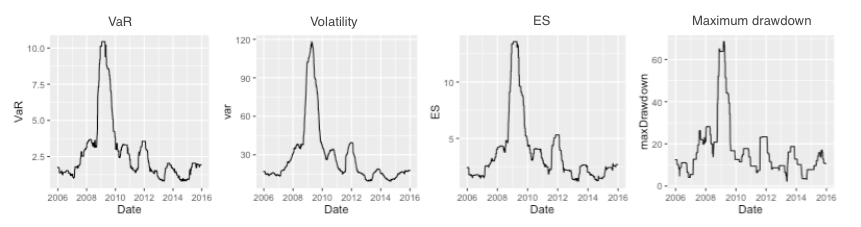
\includegraphics[width = 1\textwidth]{../results/risk_measure_RMZ}
\label{fig: risk_meausre_RMZ}
\end{figure}


\subsection{Time varying CED}

Maximum drawdown is the largest cumulative loss from peak to trough. Conditional Expected Drawdown (CED) is the tail mean of maximum drawdown distributions.\footnote{On a Convex Measure of Drawdown Risk. Lisa R. Goldberg, Ola Mahmoud} Under confidence level $\alpha$, the conditional expected drawdown is defined as:
\begin{equation}
CED_\alpha(X_{T_n}) = \textbf{E}(\mathbf{\mu}(X_{T_n})|\mathbf{\mu}(X_{T_n}) > DT_\alpha)
\end{equation}
where $\mathbf{\mu}(X_{T_n})$ is the maximum drawdown distribution over a finite path.

Here we calculated the CED using a 3-month-2-year rolling window (Figure \ref{fig: CED3mon2yr}).  Note that here we use 3 month as the basic period. For empirical distribution of 3-month maximum drawdown, there are less multi-mode problems, and the tail value is more informative than using longer period. For longer path length such as 2-year and 5-year, there might be some missing values under large confidence levels. CED data tend to be lack of variance under long time period. In such cases, the empirical quantile no longer exits without some distribution or polynomial assumption of the tail. Since we do not familiar the performance of CED, it becomes impropriate to make such assumptions. 

%%%%%
\iffalse

\begin{figure}[h]
\caption{CED under 3-month-5-year Rolling Window (confidence level = 0.95)} 
\centering 
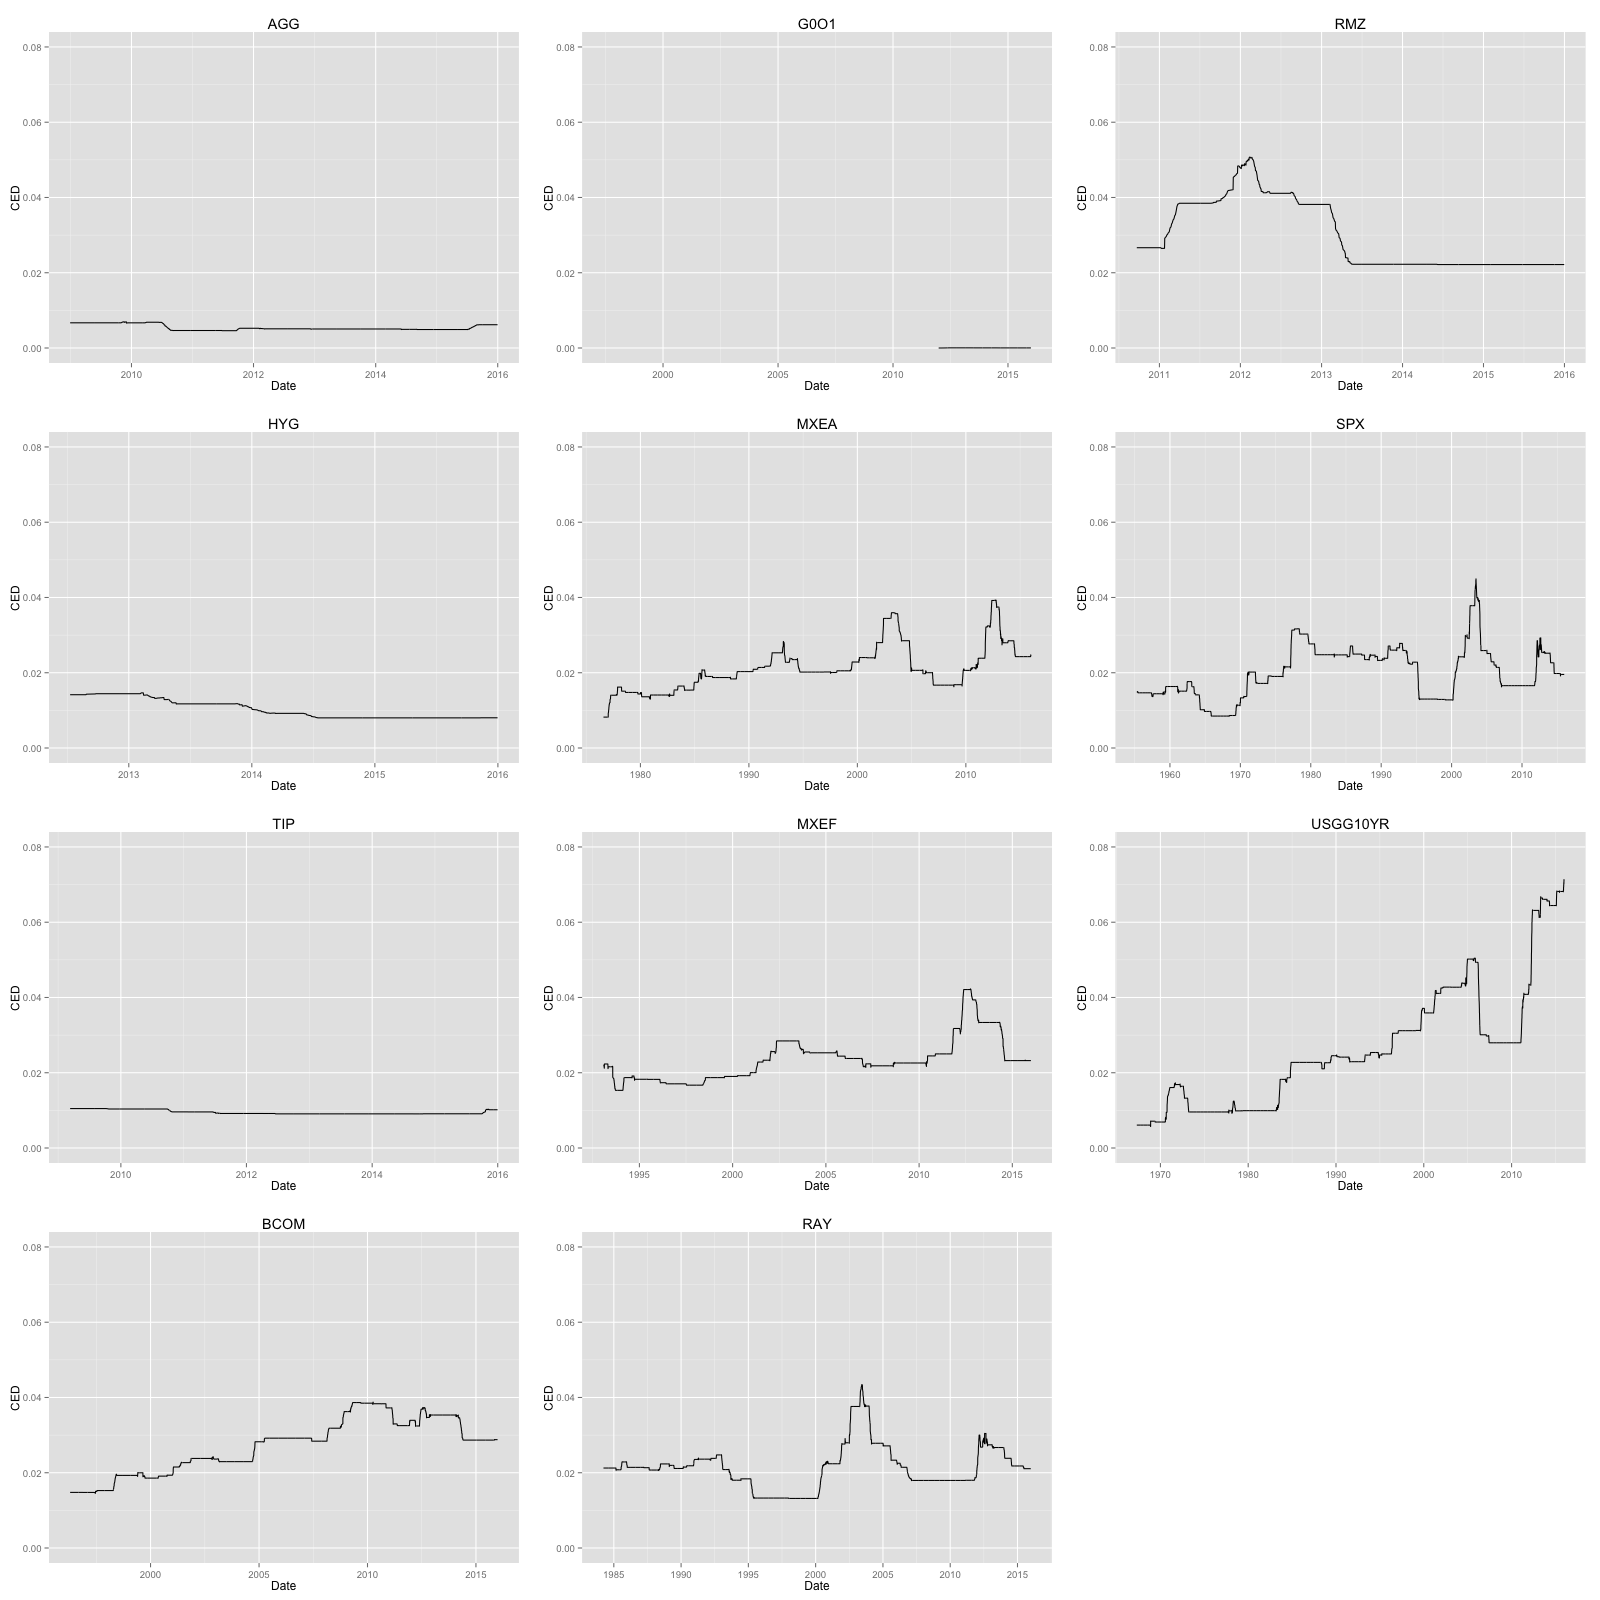
\includegraphics[width=15cm]{../results/CED_3mon_5yr_95}
\label{fig: CED3mon5yr95}
\end{figure}

\fi
%%%%%%

CED is also closely related with other traditional risk measure. However, the correlation between CED and the other three risk measures are slightly weaker than the correlation among volatility, VaR and ES. Table \ref{table:corrRiskMeasureCED} shows the correlation between CED and other risk measures. Again, the correlation is calculated based on 6-month rolling risk measures for every asset. Moreover, Figure \ref{fig: CED_ES_3mon_5yr5yr} shows the plot of ES and CED, which indicates their positive correlated relationship.


\begin{table}[!h]
\caption{Correlation between CED (confidence level = 0.9) and other risk measures}
\centering 
\begin{tabular}{ p{2cm}||p{2cm}|p{2cm}|p{2cm}} 
\hline
Measures & Volatility & VaR & ES\\
  \hline
AGG & 0.94 & 0.89 & 0.95\\ 
HYG & 0.98 & 0.97 & 0.97\\ 
TIP & 0.77 & 0.85 & 0.85\\ 
BCOM & 0.84 & 0.89 & 0.89\\ 
MXEA & 0.84 & 0.83 & 0.86\\ 
MXEF & 0.91 & 0.91 & 0.93\\ 
RAY & 0.92 & 0.85 & 0.92\\ 
RMZ & 0.96 & 0.96 & 0.97\\ 
SPX & 0.84 & 0.81 & 0.84\\ 
USGG10YR & 0.91 & 0.93 & 0.95\\
\hline
\end{tabular}
\label{table:corrRiskMeasureCED}
\end{table}

% \subsection{Time varying seirial correlation and their relationship with risk measures}


%%%%%
\iffalse

\begin{figure}[h]
\caption{CED (confidence level = 0.9) versus ES under 3-month-5-year Rolling Window} 
\centering 
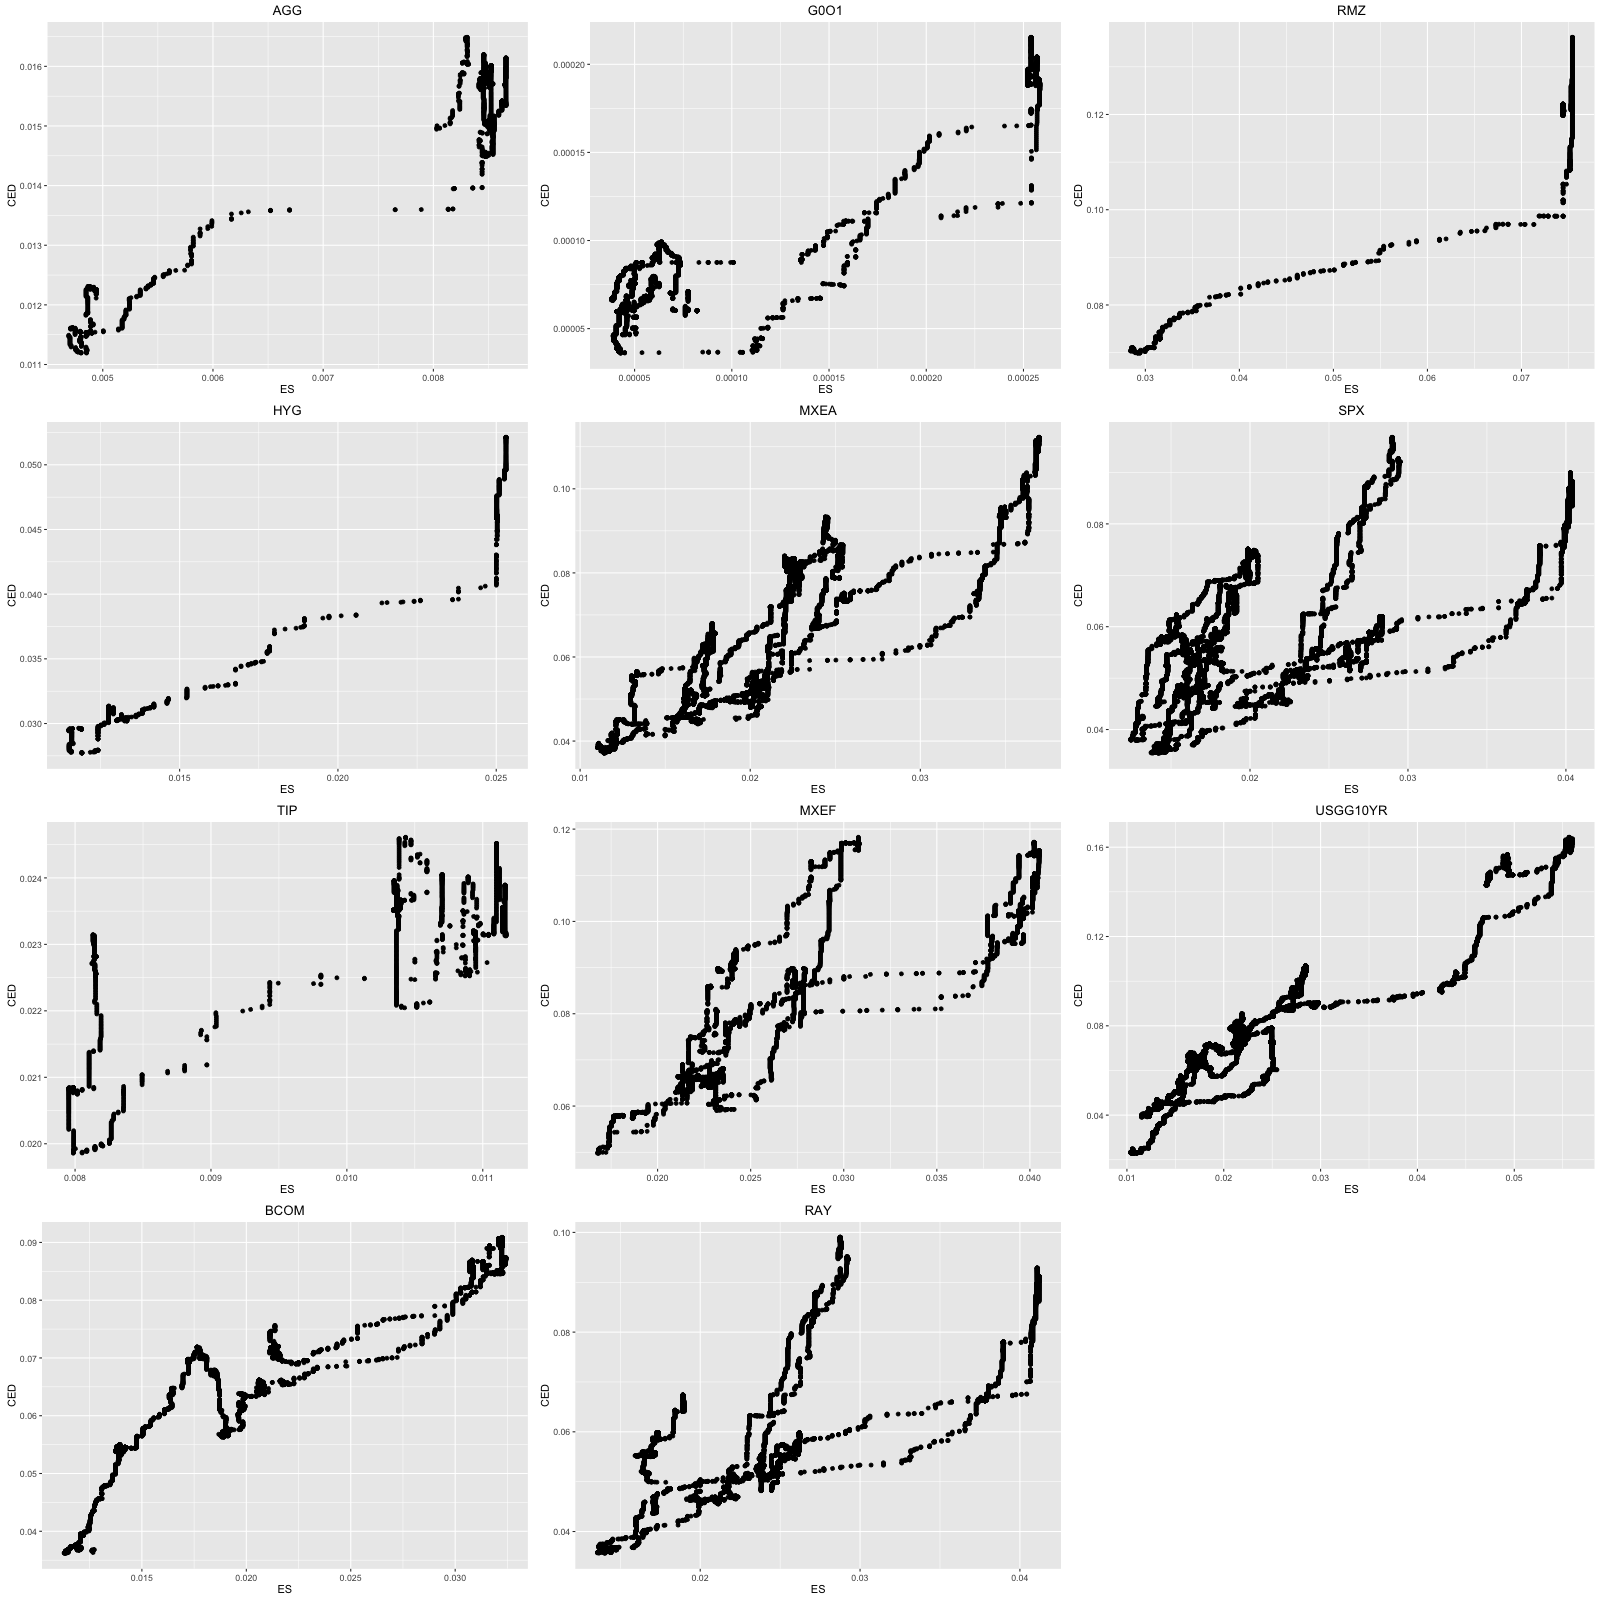
\includegraphics[width=15cm]{../results/CED_ES_3mon_5yr5yr}
\label{fig: CED_ES_3mon_5yr5yr}
\end{figure}

\fi
%%%%%%